      Logo abaixo são apresentados os resultados da primeira iteração de avaliação do protótipo de alta fidelidade,
      seguindo o planejamento realizado.
      
      \begin{itemize}
       \item \textbf{Descrição e metodologia do roteiro da avaliação}
       
       \subitem O objetivo dessa avaliação é analisar qual a satisfação obtida pelo usuário ao utilizar o protótipo 
        considerando as seguintes metas:
       
	\begin{itemize}
	  \item Utilidade;
	    \subitem Avaliada pela dimensão \textit{SysUse} do questionário PSSUQ.
	    
	  \item Eficácia e eficiência;
	    \subitem Avaliada pelas dimensões \textit{SysUse} e \textit{InfoQual} do questionário PSSUQ.
	    
	  \item Interface esteticamente agradável.
	    \subitem Avaliada pela dimensão \textit{InterQual} do questionário PSSUQ.
	\end{itemize}
       
       \item \textbf{Comportamento dos usuários}
       
	  \subitem Ao todo, os cinco usuários que avaliaram o protótipo conseguiram cumprir todas as tarefas estabelecidas 
	  de todos os cenários. Agiram perante as atividades do protótipo de maneira intuitiva, apesar de ficarem 
	  desatentos em relação a alguns ícones, e não demoraram a cumprir as funcionalidades dos cenários de avaliação 
	  estabelecidos. 
	  
	  \subitem Alguns usuários estavam com vergonha de realizar a avaliação pelo fato de ter que fazer uma gravação em vídeo. 
	  Devido a isso, foi questionado a eles se os mesmos estavam realmente seguros de realizar a avaliação ou se desejavam 
	  interromper a mesma e não realizá-la. Nessa primeira iteração, nenhum dos usuários se negaram e decidiram por 
	  continuar a avaliação
       
       \item \textbf{Resumo das entrevistas}
       
	  \subitem As entrevistas foram realizadas na prórpria universidade. EStas foram gravadas e cada uma durou em 
	  média 12 minutos contando com o tempo que o usuário teve de responder os questionários de avaliação.
	        
       \item \textbf{Problemas de usabilidade identificados}
       
	  \subitem No momento da avaliação, através de observações feitas pela equipe e por análise nos vídeos coletados,
	  foram percebidos algumas dificuldades que os usuários tiveram no momento da interação com o protótipo. São elas:
	  
	  \begin{itemize}
	  
	  \item \emph{Dificuldade em entender o significado do horário da notificação.}
	    
	    \subitem Esta dificuldade está relacionada com violação da heurística "HE10 - Ajuda e documentação" (vide seção 4.3),
	    pois não havia informações suficientes para explicar o significado do horário da notificação.
	  
	  \item \emph{Dificuldade em identificar o ícone para adicionar o tema da notificação.}
	    
	    \subitem Essa dificuldade está relacionada com a violação da heurística "HE07 - Reconhecimento em vez de memorização" (vide seção 4.3),
	    pois alguns usuários não conseguiam entender que para adicionar um tema era necessário selecioná-lo e clicar no botão de
	    adicionar. Esse problema foi ocasionado porque o botão de adicionar tema era demasiado pequeno em relação
	    aos outros componentes da tela, segundo parte dos usuários. 
	  
	  \item \emph{Dificuldade em identificar o ícone para editar uma notificação.}
	    
	    \subitem Mesmo contexto da dificuldade anterior.
	    
	  \item \emph{Dificuldade em identificar o ícone para excluir uma notificação.}
	    
	    \subitem Mesmo contexto da dificuldade anterior.
	  
	  \end{itemize}
       
       \item \textbf{Paradas críticas}
       
	  \subitem No momento da avaliação não houve nenhum caso a qual o usuário ficou sem reação em relação à execução de algum cenário. 
	  Quando os mesmos obtiveram dificuldades com alguns ícones, estes ícones foram encontrados no momento da execução.
       
       \item \textbf{Plano de correção}
       
	  \subitem Para corrigir os problemas de usabilidade que foram identificados para esta iteração, a equipe vai melhorar a
	  interface do protótipo aumentando os botões dos ícones para deixá-los mais visíveis, pois assim ficará mais intuitivo
	  para o usuário qual atividade aquele ícone vai realizar.
       
      \end{itemize}
      
      Na figura \ref{asqalta} se encontram as respostas ao questionário ASQ pelos cinco usuários avaliados.
      
      Na figura \ref{pssuqalta} se encontram as respostas ao questionário PSSUQ pelos cinco usuários avaliados.
      
      \begin{figure}[!htb]
      \centering
      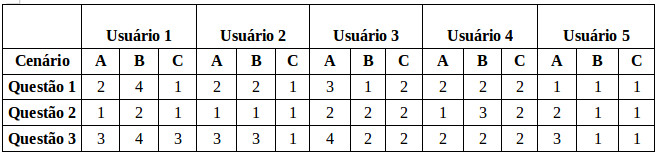
\includegraphics[scale=0.6]{figuras/asqalta.jpg}
      \caption{Resposta dos usuários ao questionário ASQ na primeira avaliação do protótipo de alta fidelidade}
      \label{asqalta}
      \end{figure}
      
      
      \begin{figure}[!htb]
      \centering
      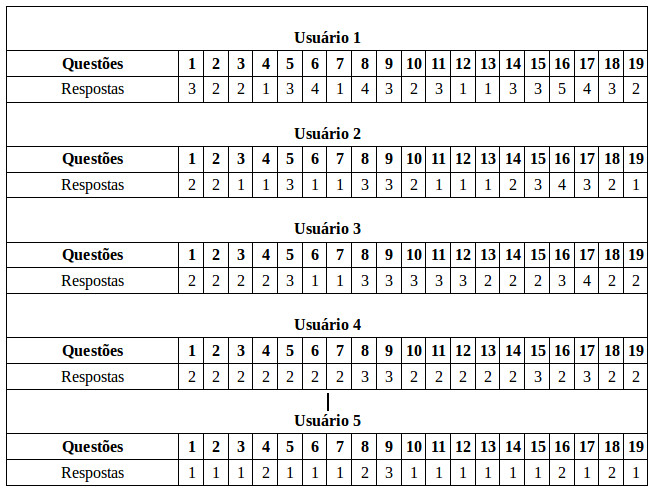
\includegraphics[scale=0.6]{figuras/pssuqalta.jpg}
      \caption{Resposta dos usuários ao questionário PSSUQ na primeira avaliação do protótipo de alta fidelidade}
      \label{pssuqalta}
      \end{figure}
